\subsubsection{Autonomus program}
 
    \begin{enumerate} 
      
      \item Sensors used in the program:
      \begin{enumerate}
      	\item HiTechnic Gyro sensor for turns and movement stabilization.
      	\item Andy's Mark encoder for range measurement.
      	\item HiTechnic RGB sensor for beacon color detection.
      \end{enumerate}
      	 
      \item Algorithm of the autonomous period:
      \begin{enumerate}
        \item Parking in the beacon zone or parking zone.
        \item Drop autonomous climbers into beacon bucket.
        \item Push the button on the beacon.
      \end{enumerate}
      
      \begin{figure}[H]
        \center{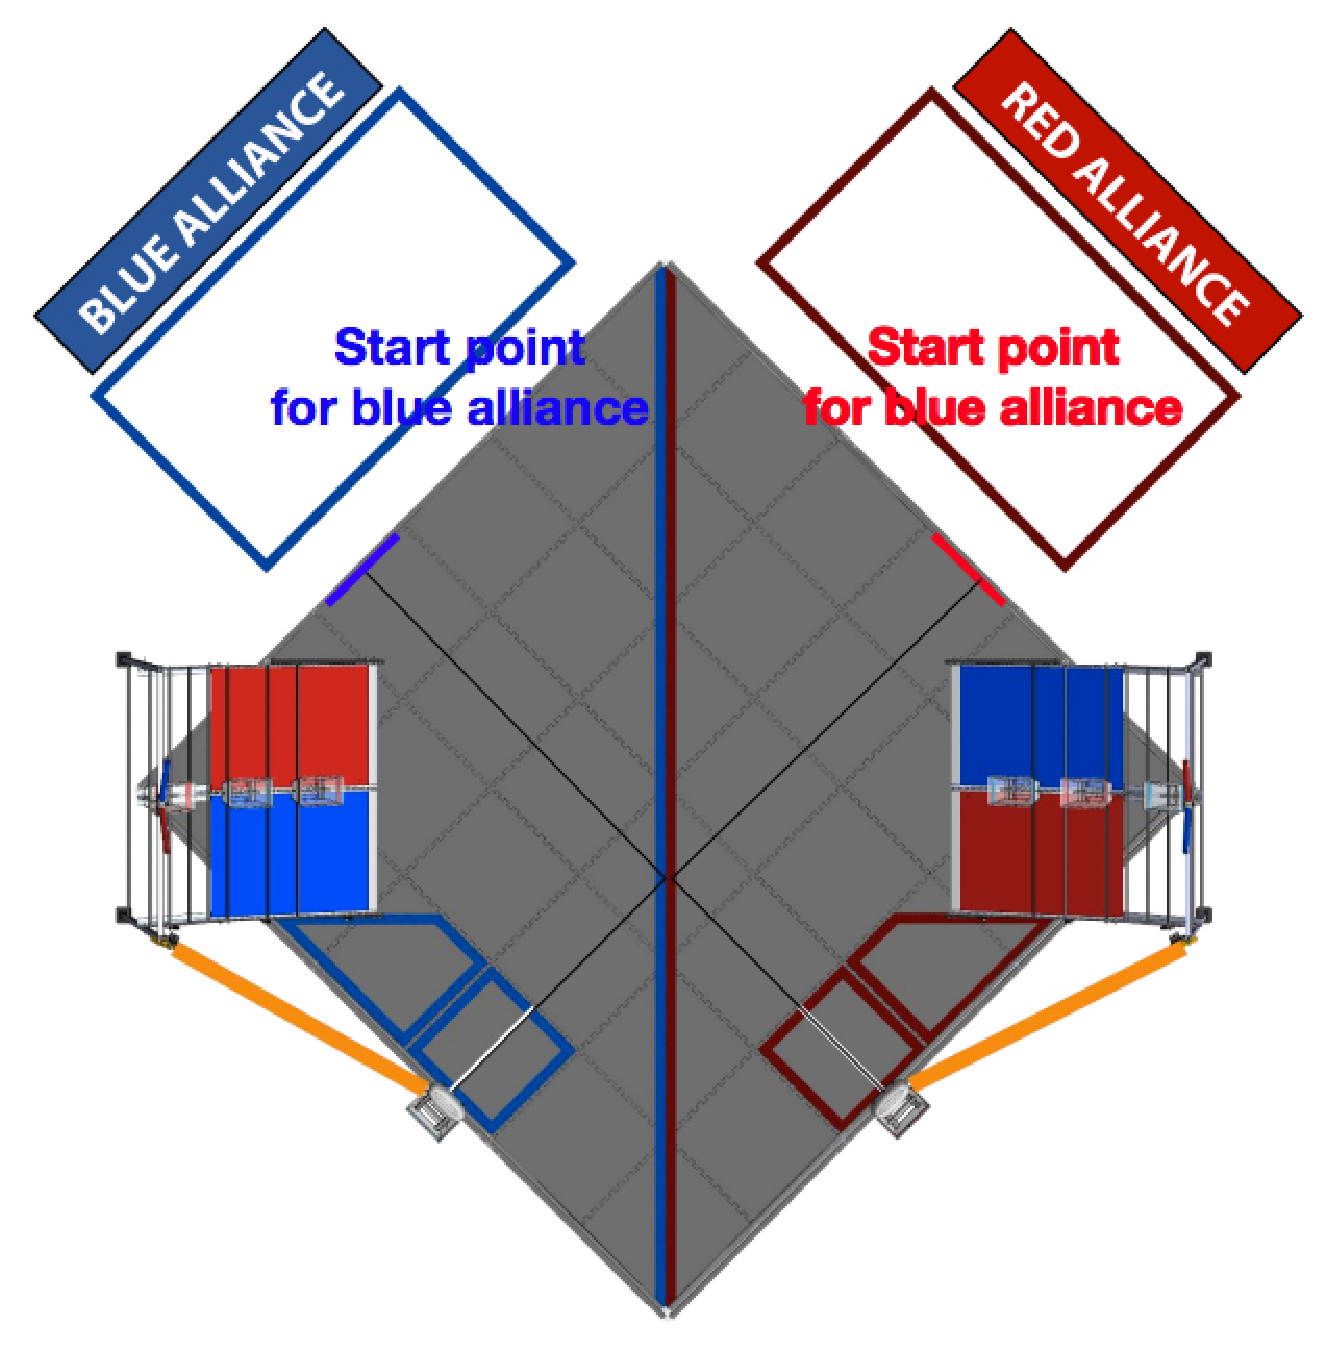
\includegraphics[scale = 0.6]{3Engineering/7Specifications_for_programmes/autonomous/images/1}}
  		\caption{Autonomous movement trajectory}
  	  \end{figure}
  	  
    \end{enumerate}  
\fillpage